\section{WORK IN PROGRESS} \label{sec:new}
Look into network discovery, for NAT.
Gå gjennom NAT?
traceroute 
Sjå på DNS tracing?
TODO: 



\subsection{Internet Protocol}
For a device connected to the internet to communicate with other devices, it needs to use an IP address. However, as the IPv4 range becomes exhausted, less devices get dedicated IPv4 addresses. To be able to connect these, several solutions are used. The two most popular are IPv6 and Network address translation (NAT).
IPv6 has enough IP addresses for the foreseeable future. However, the internet has not yet fully changed to using IPv6. Shodan has crawlers for the IPv6 address space.
NAT lets you connect multiple devices to the same IPv4. This is done by using a routing device with a shared IPv4 address to receive packages for multiple different devices, and then redirect the packages to the correct receiver. This makes it so that the devices behind the NAT can reach the internet, while the internet can not reach the devices unless the devices start the communication. Because of this, Shodan will only scan the outer NAT routing device, and not the devices behind the NAT. NAT is not always used for getting more IPv4 addresses. Sometimes it is used purposely to hide IPv4 addresses from the public internet.


\section{Methodology}
The Interned is designed to connect people and things across the globe. With good tools like Shodan, it is easy to find different online devices. The challenge is to identify these devices. This becomes more difficult the more specific the identification needs to be. The Shodan banners mentioned before is a good place to find this. Another method is to find an Internet Service Provider that operates in a specific industry, and find its IP range. The Shodan banners also contain a geographical location, and this might be used to find offshore systems.

\subsection{Banner similarities}
When connecting a device to the internet, it needs to be configured. The installer needs competence to do this properly, and to spend time to perform the installation. To make such devices more accessible and efficient, finished solutions are most often used. Due to this, the same devices mostly have the same default configuration, and therefore the same banners. This can be used to identify devices within the chosen constraints by using the following method.
\begin{enumerate}
    \item Identify a device fulfil the constraints and is connected to the internet.
    \item Find the IP address of said device, and find its Shodan entry.
    \item Get its banner.
    \item Use unique information from the banner to find all devices with similar banners.
\end{enumerate}
The most difficult of these steps is to find the IP address. The easiest way to do this is to own a device and find its IP address. Unfortunately, this project does not have access to any devices that fit the constraints set.
If this is not an option, the device would be found by guessing what information could be found in its banner, for example the device name or ports it has open.

\subsection{Internet Service Provider}
Internet Service Providers(ISP) are the organisations that connect people and companies to the internet. ISP charges money to deliver internet connection, and most people have a subscription. While a lot of ISPs are generalized, and deliver the internet to both private and organizational customers, others are more specialized. If it is possible to find any ISP that only delivers to the groups defined in the constraints, Shodan can filter IP addresses based on ISP .

\subsection{IP range}
IP addresses are commonly divided into ranges using Classless Inter-Domain Routing(CIDR). These IP ranges are owned by different companies. Often, it is the ISP that owns IP ranges. However, large enough companies sometimes own their own IP addresses. If a company with an IP range is within the search constraints, it could be possible to find the IP range of said company, and then use the Shodan filter "net" to find all IPs in the range that is connected.

\begin{figure}
    \centering

    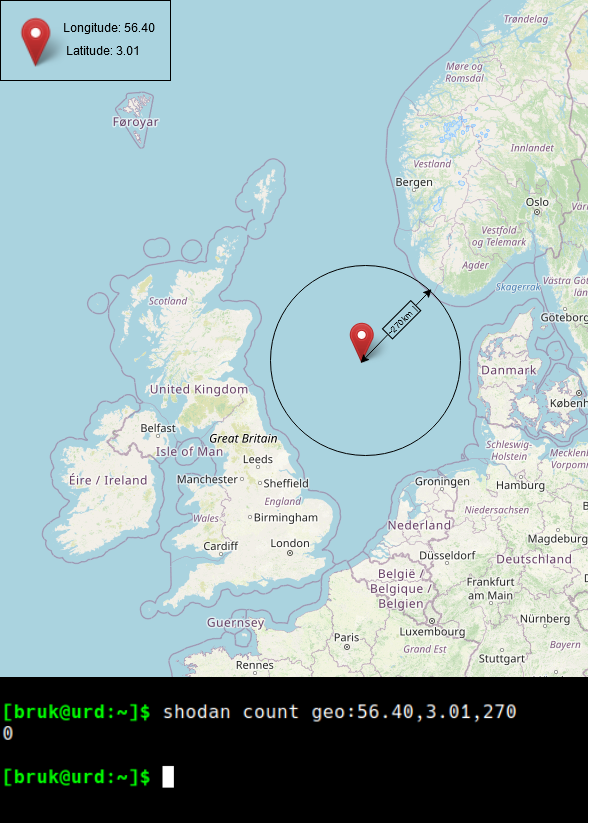
\includegraphics[scale=0.7]{Figurer/geolocation.png}
    \caption{Shodan "geo" filter visualized. Map copyright: https://www.openstreetmap.org/copyright}
    \label{fig:api_doc}
\end{figure}